\documentclass[9pt]{article}

\usepackage{graphicx}
\usepackage{ragged2e}
\usepackage{geometry}
    \geometry{a4paper,
    margin=0.25in}
\usepackage{lettrine}
\usepackage{fontspec}
\setmainfont{Miller-TextRoman.otf}

\newfontface\headlinefont{Miller-DisplayRoman.otf}[Contextuals={WordInitial,WordFinal}]


\begin{document}
\noindent
%\begin{minipage}[t]{0.55\textwidth}
{\headline\fontsize{37}{30}\bfseries Young Voter Registration Saw Increase Ahead of 2024 Elections}
%\end{minipage}

\vspace{3pt}

\noindent
\begin{minipage}{0.45\textwidth}
    \begin{justify}
% text with drop cap top left section
    \lettrine[lines=3, lraise=0]{I}n the lead-up to the UK’s local elections on 2 May 2024, voter registration numbers saw a significant uptick, particularly among young people. The surge, which occurred about two weeks prior to the election, was repeated later in the summer just before the general election on 4 July 2024. In mid-June, the number of newly registered voters in one day reached a high for the year with well over 600,000 voter registrations. Both peaks this summer were, unsurprisingly, driven largely by an influx of young voters. \\
 Young people under 25, along with those in the 25-34 age group, accounted for most of the new voter registrations, with these two categories collectively representing an astounding 56\% of all new voters in 2024. Although registration numbers cannot reveal the demographics of those voters who did turnout, the large number of new registrants shows high engagement among younger people. In particular, the share of new voters in the 25-34 age group, people that would have been eligible to vote for at least the last two general elections (in 2017 and 2019), indicates that this year’s elections may have inspired more participation than previous cycles.\\
     This surge in registration may signal a growing political awareness among younger generations, who are increasingly motivated by issues such as the cost of living, healthcare access, and social justice. It also suggests that young voters are becoming a more influential force in shaping the outcome of elections. The challenge now for political parties will be to ensure that these newly registered voters are not only mobilised but also motivated to turn out on polling day, translating registration numbers into tangible votes. Whether this trend marks a permanent shift in youth political engagement remains to be seen.

    \end{justify}
\end{minipage}%
\hspace{0.05\textwidth}
% stacked images on right
\begin{minipage}[t]{0.45\textwidth}
  \includegraphics[width=\linewidth]{ages_pie.jpeg}
  
  \vspace{5pt} 
  
  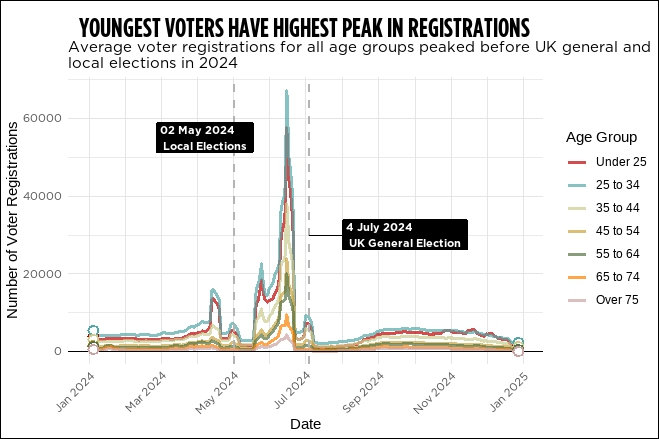
\includegraphics[width=1.1\linewidth]{age_lines_w_callouts.jpeg}
\end{minipage}

\vspace{3pt}

% full image
\begin{center}
  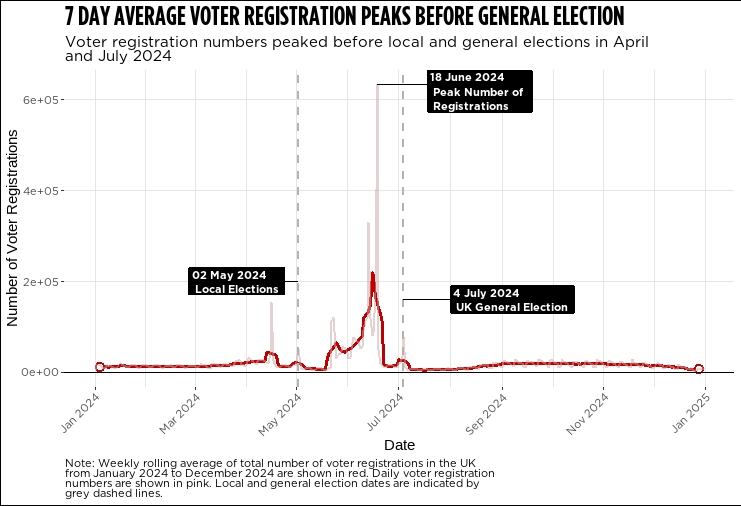
\includegraphics[width=0.95\textwidth, height=11cm]{daily_registrations.jpeg}
\end{center}

\end{document}
